\def\year{2015}
\documentclass[letterpaper]{article}

\usepackage{aaai}
\usepackage{times}
\usepackage{helvet}
\usepackage{courier}

\usepackage{graphicx}
\usepackage{amsmath}
\usepackage{amssymb}
\usepackage{amsthm}

\usepackage{algorithm}
\usepackage{algpseudocode}

\frenchspacing
\setlength{\pdfpagewidth}{8.5in}
\setlength{\pdfpageheight}{11in}

\pdfinfo{
/Title (Insert Your Title Here)
/Author (Put All Your Authors Here, Separated by Commas)}

\setcounter{secnumdepth}{0}  

\input{macros}
\usepackage[textsize=footnotesize,color=green!40]{todonotes}
\newcommand{\borja}[1]{\todo[inline,color=green!40]{{\it Borja:~}#1}}
\newcommand{\doina}[1]{\todo[inline,color=red!40]{{\it Doina:~}#1}}
\newcommand{\lucas}[1]{\todo[inline,color=blue!40]{{\it Lucas:~}#1}}

\begin{document}

\title{Learning Multi-Step Predictive State Representations - Appendix}
%\author{Anonymous Submission}
\maketitle

\begin{abstract}
\begin{quote}
This appendix contains pseudocode for the algorithms presented in the main paper, and more details on the experiments.

\end{quote}
\end{abstract}

\section{Pseudocode of the encoding function}

The pseudocode is given in Algorithm 1, using the following notation:

\textbf{bestEncoding}: A map from indices i of Q to the optimal encoding of Q[:i].

\textbf{minEncoding}: A map from indices i of Q to $|bestE[i]|$

\textbf{opsEnding}: A map from indices i of Q to the set of strings in $\Sigma'$: $\{x \in \Sigma' s.t Q[i-|x|:i] == x\}$

\algnewcommand\algorithmicinput{\textbf{INPUT:}}
\algnewcommand\algorithmicoutput{\textbf{OUTPUT:}}

\algnewcommand\INPUT{\item[\algorithmicinput]}
\algnewcommand\OUTPUT{\item[\algorithmicoutput]}

\begin{algorithm}
\caption{Encoding Algorithm}
\label{Encoding Algorithm}
\begin{algorithmic}[1]
\INPUT $x$
\OUTPUT $\kappa(x)$

\Procedure{DPEncode}{}

\State $bestEncoding[] \gets String[|x|+1]$
\State $minEncoding[] \gets Int[|x|+1]$
\State $opsEnding[] \gets String[|x|+1][]$

\State $bestEncoding[0] = x[0]$
\State $minEncoding[0] = 0$

\For{i in $[1,|x|]$}
	 \State $ospEnding[i] \gets \{s \in \Sigma', x[i-|s|:i] == s\}$
\EndFor

\For{i in $[1,|x|]$}
	\State $bestOp \gets null$
	\State $m \gets null$ 
	\For{$s \in opEnd[i]$}
		\State $t \gets minE[i-|s|] + 1$
		\If{$m == null$ or $t < m$}
			\State $m \gets t$ 
			\State $bestOp \gets s$
		\EndIf
	\EndFor
	\State $minEncoding[i+1] \gets m$
	\State $bestEncoding[i+1] \gets bestEncoding[i-|bestOp|] + bestOp$
\EndFor

\State \Return $bestEncoding[|x|]$

\EndProcedure
\end{algorithmic}
\end{algorithm}

\begin{algorithm}
\caption{Base Selection Algorithm}
\label{Base Selection Algorithm}
\begin{algorithmic}[1]
\INPUT $Train$, $Sub_M$
\OUTPUT $\Sigma'$

\Procedure{Base Selection}{}
\State $\Sigma' \gets \{s, s \in \sum \}$

\State $bestEncoding \gets null$
\For{each obs in Train}
	\State $bestEncoding[obs] \gets |obs|$
\EndFor

\State $i \gets 0$\
\While{$i<numOps$}
	\State $bestOp \gets null$
	\State $m \gets 0$
	\For{each s $\in Sub_M$ }
		\State $c \gets 0$
		\For{each obs in Train}
			\State $c \gets c+DPEncode(obs)-prevBestE(obs)$
		\EndFor
		
		\If{$c>m$}
			\State $bestOp \gets obs$
			\State $m \gets c$
		\EndIf
		
	\EndFor

	\State $\Sigma' \gets \Sigma' \cup bestOp$
	\For{each obs in Train}
		\State $bestEncoding \gets DPEncode(obs,\Sigma'$) 
	\EndFor	
	
	\State $i \gets i + 1$
\EndWhile 
\State \Return $\Sigma'$

\EndProcedure
\end{algorithmic}
\end{algorithm}

\newpage

\section{Experiments}

The figures below depict the Double Loop and Pacman environments used in the experiments.

\begin{figure}[ht!]
\centering

\includegraphics[width=60mm]{uCOREPICS/DL/doubleLoopImage.png}
\caption{Double Loop Environment\label{overflow}}
\end{figure}

\begin{figure}[ht!]
\centering
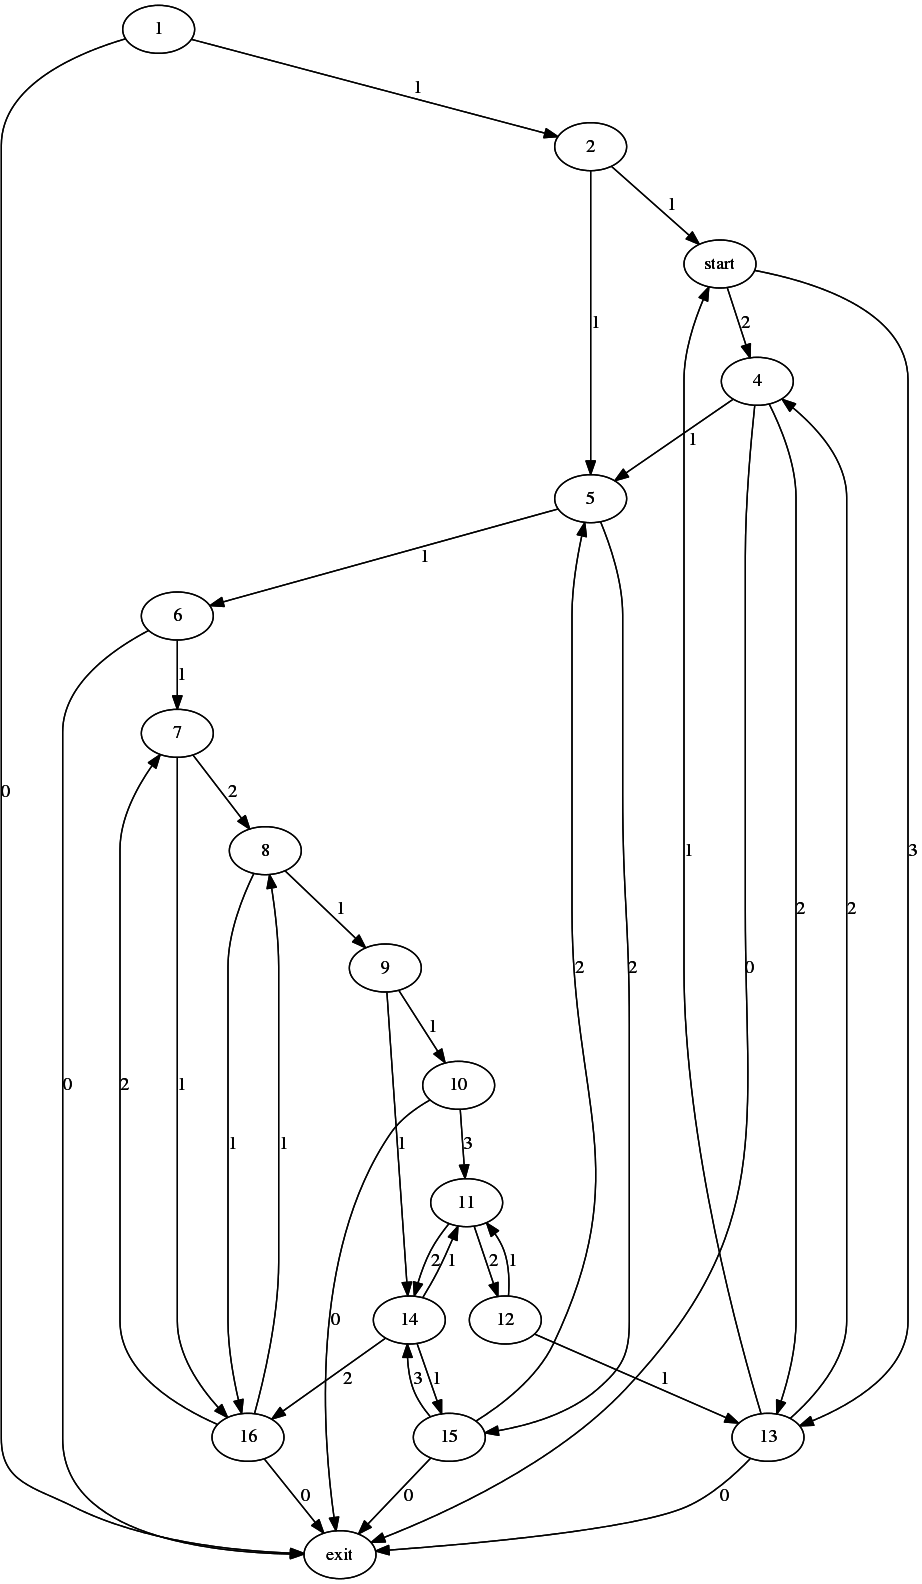
\includegraphics[width=40mm,height=60mm]{uCOREPICS/Pacman/graphPacMan.png}
\caption{Graph of Pacman Labyrinth\label{overflow}}
\end{figure}


\end{document}